% !TeX root = main.tex
% !TEX program = pdflatex

\chapter{Sensores Generadores}\label{cap:generadores}

A diferencia de los sensores pasivos (resistivos y reactivos), los sensores generadores transforman directamente la energía del mensurando en energía eléctrica sin necesidad de una fuente de alimentación externa para la transducción. En este capítulo analizaremos los dos grupos más relevantes en la industria: los termopares, basados en efectos termoeléctricos, y los sensores piezoeléctricos, basados en la generación de carga por deformación mecánica.


\section{Sensores Termoeléctricos: Termopares}\label{sec:termopares}
Los termopares son los sensores de temperatura más utilizados en la industria debido a su robustez, bajo coste y, especialmente, su amplísimo rango de medida (desde \qty{-200}{\degree C} hasta más de \qty{2000}{\degree C}). Su funcionamiento se basa en la termoelectricidad, un fenómeno donde la energía térmica se convierte en potencial eléctrico. 

\subsection{Fundamentos Físicos: Efectos Seebeck, Peltier y Thomson}
\paragraph{El Efecto Seebeck}
El principio físico subyacente es el \emph{efecto Seebeck}, descubierto en 1821. Como se muestra en la figura \ref{fig:seebeck_principio}, cuando dos conductores de materiales distintos ($A$ y $B$) se unen en sus extremos formando un lazo, y existe una diferencia de temperatura entre las uniones, aparece una fuerza electromotriz (f.e.m.) que induce una corriente.

\begin{marginfigure}[2em]
    \centering
    \shorthandoff{>}
    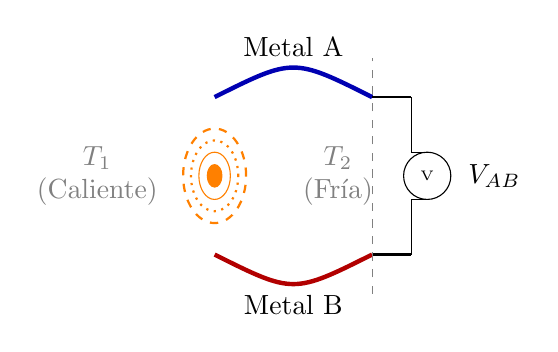
\begin{tikzpicture}[scale=1, >=stealth]
        % Material A
        \draw[ultra thick, blue!70!black] (0,2) .. controls (1,2.5) .. (2,2) node[midway, above, black] {Metal A};
        % Material B
        \draw[ultra thick, red!70!black] (0,0) .. controls (1,-0.5) .. (2,0) node[midway, below, black] {Metal B};
        
        % Unión caliente T1 con efecto irradiante (elipses concéntricas)
        \begin{scope}[shift={(0,1)}]
            % Elipse central (el núcleo caliente)
            \fill[orange] (0,0) ellipse (0.1cm and 0.15cm);
            % Elipses concéntricas con diferentes estilos para el efecto irradiante
            \draw[orange, dashed, thick] (0,0) ellipse (0.4cm and 0.6cm);
            \draw[orange, dotted, thick] (0,0) ellipse (0.3cm and 0.45cm);
            \draw[orange, thin] (0,0) ellipse (0.2cm and 0.3cm);
        \end{scope}
        \node[left, gray, align=center] at (-0.6,1) {$T_1$ \\ (Caliente)};
        
        % Conexión al voltímetro
        \draw[thick] (2,2) -- (2.5,2);
        \draw[thick] (2,0) -- (2.5,0);
        \draw (2.7,1) circle (0.3) node[font=\tiny] {V};
        \draw (2.5,2) |- (2.7,1.3);
        \draw (2.5,0) |- (2.7,0.7);
        
        \node[right] at (3.1,1) {$V_{AB}$};
        \node[right, gray, align=center] at (1,1) {$T_2$ \\ (Fría)};
        \draw[dashed, gray] (2,-0.5) -- (2,2.5);
    \end{tikzpicture}
    \caption{Lazo termoeléctrico básico. La tensión de Seebeck $V_{AB}$ es proporcional a la diferencia de temperatura entre la unión de medida ($T_1$) y la unión de referencia ($T_2$).}\label{fig:seebeck_principio}
\end{marginfigure}

\marginnote{\textbf{Nota Histórica:} Thomas Seebeck descubrió el efecto de forma accidental al observar que una aguja de brújula se desviaba cerca de un lazo de dos metales con distinto gradiente térmico, confundiéndolo inicialmente con un fenómeno magnético.
}

Físicamente, esto ocurre porque la densidad de electrones libres en un conductor depende de la temperatura. Al calentar un extremo, los electrones adquieren energía cinética y migran hacia la zona fría, creando un potencial electrostático. Como cada metal tiene una \emph{afinidad} distinta por sus electrones (función de trabajo), la magnitud de este desplazamiento es diferente en el metal A y en el metal B, resultando en una diferencia de potencial neta.

La tensión de circuito abierto $V_{AB}$ generada es proporcional a la diferencia de temperatura entre la unión caliente ($T_h$) y la unión fría o de referencia ($T_c$):

\begin{equation}\label{eq:seebeck_integral}
    V_{AB} = \int_{T_c}^{T_h} (\alpha_A(T) - \alpha_B(T)) \, dT
\end{equation}

Donde $\alpha_A$ y $\alpha_B$ son los \emph{coeficientes de Seebeck} de cada material (medidos en \unit{\mu V/\degree C}). Para variaciones de temperatura moderadas, los coeficientes se consideran constantes y la relación se simplifica a:

\begin{equation}\label{eq:seebeck_lineal}
    V_{AB} \approx \alpha_{AB} \cdot (T_h - T_c)
\end{equation}

Aquí, $\alpha_{AB}$ es la \emph{sensibilidad del termopar}. Es fundamental recalcar que un termopar \emph{no mide temperatura absoluta}, sino la diferencia de temperatura entre dos puntos. Para conocer $T_h$, es imperativo conocer con precisión la temperatura de la unión de referencia $T_c$.

\paragraph{Efectos Peltier y Thomson}
Aunque el efecto Seebeck es el aprovechado para la sensórica, existen otros dos efectos relacionados en la termoelectricidad:
\begin{itemize}
    \item \emph{Efecto Peltier}: Descubierto por Jean Peltier en 1834. Es el inverso del Seebeck: al hacer circular corriente, la unión absorbe o libera calor.
    \item \emph{Efecto Thomson}: Predicho por William Thomson (Lord Kelvin) en 1854 mediante termodinámica, describe el intercambio de calor en un único conductor con gradiente térmico.
\end{itemize}

\marginnote{\textbf{Peltier y Lenz:} El efecto Peltier fue tan sorprendente que el físico Emil Lenz tuvo que demostrarlo en 1838 congelando agua en una unión de bismuto y antimonio para convencer a los escépticos de la época.}

\marginnote{\textbf{La síntesis de Kelvin:} Lord Kelvin unificó la termoelectricidad en su obra \textit{On the Dynamical Theory of Heat}, demostrando que Seebeck y Peltier eran dos caras de la misma moneda termodinámica.}

\begin{marginfigure}
    \centering
    \shorthandoff{>}
    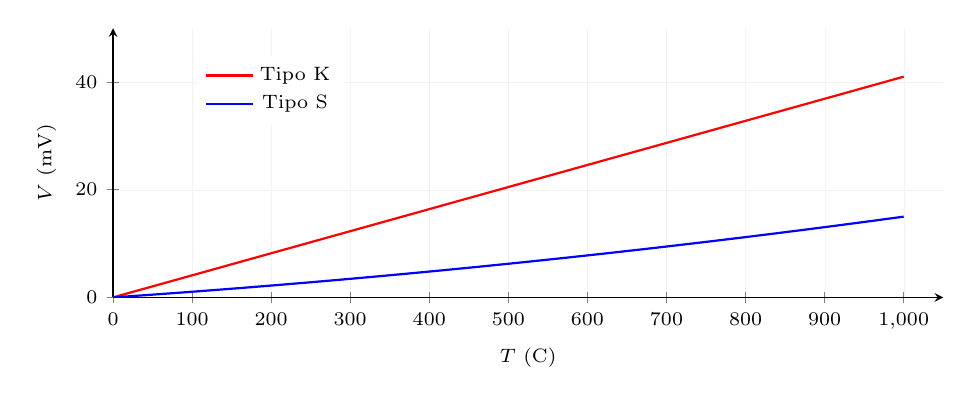
\begin{tikzpicture}
        \begin{axis}[
            width=\linewidth, height=5cm,
            xlabel={$T$ (\unit{\degree C})}, ylabel={$V$ (\unit{mV})},
            xmin=0, xmax=1050, ymin=0, ymax=50,
            axis lines=left, grid=both,
            grid style={line width=.1pt, draw=gray!10},
            font=\scriptsize,
            legend style={at={(0.1,0.9)}, anchor=north west, draw=none}
        ]
            % Tipo K (Chromel-Alumel) aprox 41 uV/C
            \addplot[thick, red, domain=0:1000] {0.041*x};
            \addlegendentry{Tipo K}
            % Tipo S (Platino-Rodio) aprox 10 uV/C
            \addplot[thick, blue, domain=0:1000] {0.010*x + 0.000005*x^2};
            \addlegendentry{Tipo S}
        \end{axis}
    \end{tikzpicture}
    \caption{Curvas de respuesta para termopares estándar. El tipo K es casi lineal y sensible, mientras que el tipo S (metales nobles) es menos sensible pero extremadamente estable a altas temperaturas.}\label{fig:curvas_termopares}
\end{marginfigure}


\subsection{Leyes de los Circuitos Termoeléctricos}
Para el diseño de sistemas de medida, el ingeniero debe aplicar tres leyes fundamentales que permiten manipular los cables sin introducir errores:

\begin{enumerate}
    \item \emph{Ley de los Metales Intermedios}: Si se inserta un tercer metal $C$ en cualquier punto de un circuito termoeléctrico, la f.e.m. total no varía siempre que las dos nuevas uniones creadas estén a la misma temperatura. Esto permite soldar los termopares o conectarlos a bornes de cobre.
    \item \emph{Ley de las Temperaturas Intermedias}: La f.e.m. producida entre $T_1$ y $T_3$ es la suma algebraica de las f.e.m. producidas entre $T_1, T_2$ y las de $T_2, T_3$. Esto facilita la calibración y el uso de tablas referenciadas a \qty{0}{\degree C}.
\end{enumerate}

\marginnote{\textbf{Importancia del Aislamiento:} En la fabricación de termopares, los hilos deben estar aislados eléctricamente entre sí en toda su longitud, excepto en la unión de medida (punta caliente). Un cortocircuito accidental en cualquier otro punto crearía una "nueva unión" y la medida correspondería a la temperatura de ese punto de fallo.
}

\subsection{Tipos de Termopares y Rangos (Normativa IEC)}

Las combinaciones de metales para formar termopares han sido estandarizadas internacionalmente por normas como la \emph{IEC 60584} o la ANSI MC96.1. Cada tipo se identifica por una letra y posee características de sensibilidad y resistencia ambiental específicas como se muestra en la Tabla~\ref{tab:tipos_termopares} y en la Figura~\ref{fig:curvas_termopares}.

\paragraph{Clasificación General}
Los termopares se dividen fundamentalmente en dos grupos:
\begin{enumerate}
    \item \emph{Metales Básicos}: Tipos J, K, T, E y N. Son económicos y poseen una sensibilidad elevada (típicamente \qtyrange{40}{60}{\mu V/\degree C}).
    \item \emph{Metales Nobles}: Tipos R, S y B. Basados en Platino y Rodio. Son costosos, pero extremadamente estables a muy altas temperaturas y resistentes a la oxidación. Su sensibilidad es baja (\qty{10}{\mu V/\degree C}).
\end{enumerate}

\begin{table}[ht]
    \centering
    \small
    \caption{Características de los termopares estándar según IEC. Los valores de sensibilidad son promedios en sus rangos lineales.}\label{tab:tipos_termopares}
    \setlength{\tabcolsep}{15pt}
    \begin{tabularx}{\linewidth}{c X c c}
        \toprule
        \textbf{Tipo} & \textbf{Materiales (+ / -)} & \textbf{Rango (\qty{}{\degree C})} & \textbf{Sensibilidad} \\
        \midrule
        \emph{K} & Chromel / Alumel & \num{-200} a \num{1250} & \qty{41}{\mu V/\degree C} \\
        \emph{J} & Hierro / Constantán & \num{0} a \num{750} & \qty{52}{\mu V/\degree C} \\
        \emph{T} & Cobre / Constantán & \num{-200} a \num{350} & \qty{43}{\mu V/\degree C} \\
        \emph{E} & Chromel / Constantán & \num{-200} a \num{900} & \qty{68}{\mu V/\degree C} \\
        \emph{N} & Nicrosil / Nisil & \num{-200} a \num{1300} & \qty{39}{\mu V/\degree C} \\
        \emph{S} & Pt-10\%Rh / Pt & \num{0} a \num{1450} & \qty{10}{\mu V/\degree C} \\
        \bottomrule
    \end{tabularx}
\end{table}

\paragraph{Termopar Tipo K (El estándar universal)}
Es el más utilizado en la industria general debido a su amplio rango y buena resistencia a la oxidación. Sin embargo, no debe utilizarse en atmósferas reductoras sin protección, ya que el cromo puede sufrir un fenómeno de "corrosión verde" que altera la calibración.

\paragraph{Termopar Tipo J (Económico)}
Muy popular en maquinaria de inyección de plásticos. Su principal limitación es el hierro, que se oxida rápidamente por encima de los \qty{750}{\degree C}, lo que limita su vida útil en ambientes húmedos u oxidantes.

\paragraph{Termopar Tipo T (Precisión y Criogenia)}
Es el único que utiliza cobre en uno de sus hilos, lo que facilita enormemente la conexión a los terminales de medida. Es el preferido en aplicaciones biomédicas y criogénicas por su excelente estabilidad en el rango de \qty{-200}{\degree C} a \qty{200}{\degree C}.

\begin{marginfigure}
    \centering
    \shorthandoff{>}
    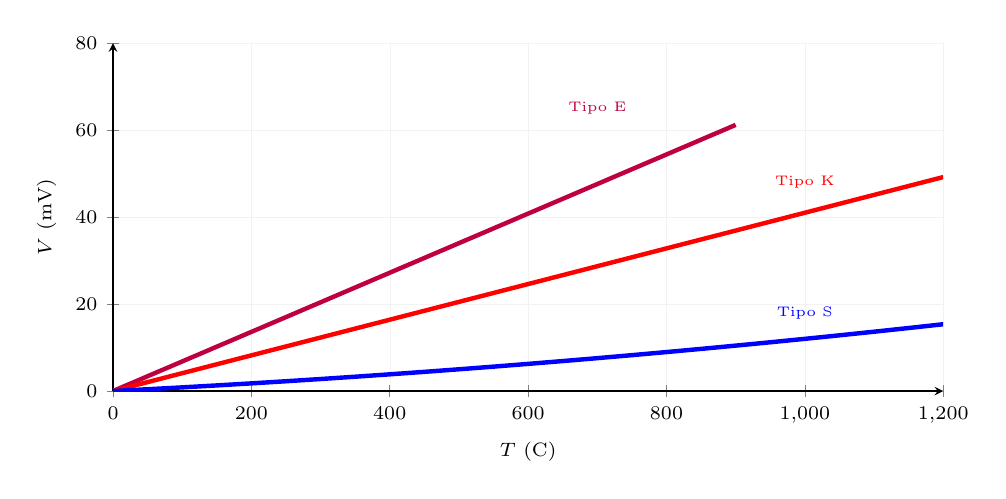
\begin{tikzpicture}
        \begin{axis}[
            width=\linewidth, height=6cm,
            xlabel={$T$ (\unit{\degree C})}, ylabel={$V$ (\unit{mV})},
            xmin=0, xmax=1200, ymin=0, ymax=80,
            axis lines=left, grid=both,
            grid style={line width=.1pt, draw=gray!10},
            font=\scriptsize,
            legend style={at={(0.05,0.95)}, anchor=north west, font=\tiny, draw=none}
        ]
            % E: ~68uV/C
            \addplot[ultra thick, purple, domain=0:900] {0.068*x};
            \node[purple, font=\tiny] at (axis cs:700, 65) {Tipo E};
            
            % K: ~41uV/C
            \addplot[ultra thick, red, domain=0:1200] {0.041*x};
            \node[red, font=\tiny] at (axis cs:1000, 48) {Tipo K};
            
            % S: ~10uV/C (más curvado)
            \addplot[ultra thick, blue, domain=0:1200] {0.008*x + 0.000004*x^2};
            \node[blue, font=\tiny] at (axis cs:1000, 18) {Tipo S};
        \end{axis}
    \end{tikzpicture}
    \caption{Comparativa de salida de tensión. El Tipo E ofrece la mayor relación señal-ruido, mientras que el Tipo S se reserva para aplicaciones donde la estabilidad es prioritaria sobre la amplitud de señal.}\label{fig:comparativa_mv}
\end{marginfigure}

\marginnote{\textbf{Código de Colores:} 
    A diferencia de las resistencias, los termopares se identifican por el color de sus fundas. \emph{IEC}: El positivo es siempre el color del termopar y el negativo es \emph{blanco}. \emph{ANSI}: El negativo es siempre \emph{rojo}. Esta confusión de estándares es una causa común de errores de polaridad en el laboratorio.
}

\paragraph{Termopares de Metales Nobles (R, S y B)}
Se utilizan exclusivamente en laboratorios de calibración y procesos de fundición de vidrio o acero. Su elevado coste se justifica por su inmunidad a la contaminación química y su capacidad de mantener la precisión a temperaturas extremas, aunque su sensibilidad sea inferior como se muestra en Figura~\ref{fig:comparativa_mv}).

\marginnote{\textbf{Linealidad:} Ningún termopar es perfectamente lineal. Los instrumentos modernos almacenan polinomios de orden 9 (ITS-90) para realizar la conversión de \unit{mV} a \unit{\degree C} con errores de milésimas de grado.
}



\subsection{Compensación de la Unión Fría (CJC)}\label{sec:cjc}
% Aquí es vital explicar la necesidad de un sensor adicional (NTC o Pt100) en el conector.

Como se ha analizado anteriormente, un termopar genera una tensión proporcional a la \emph{diferencia de temperatura} entre sus dos uniones. Matemáticamente:
\begin{equation}
    V_{out} = \alpha (T_{medida} - T_{ref})
\end{equation}
Para obtener la temperatura absoluta $T_{medida}$, es imprescindible conocer con exactitud la temperatura del punto donde los cables del termopar se conectan al instrumento de medida (normalmente bornes de cobre). Este punto se denomina \emph{Unión Fría} o de referencia ($T_{ref}$).

\paragraph{El Bloque Isotérmico}
En la práctica, los terminales de conexión del instrumento se montan sobre una pieza de material con alta conductividad térmica pero aislante eléctrico, denominada bloque isotérmico. Como se muestra en la Figura~\ref{fig:bloque_isotermico}, el objetivo es garantizar que ambas conexiones (el hilo positivo y el negativo) se encuentren exactamente a la misma temperatura $T_{ref}$, evitando que aparezcan gradientes térmicos parásitos que falsearían la medida.

Dentro del bloque isotérmico se coloca un sensor de temperatura auxiliar (típicamente una NTC o un RTD) que mide $T_{ref}$ con precisión. Esta información es crucial para realizar la compensación de la unión fría, ya sea por software o por hardware, y así obtener una medida correcta de $T_{medida}$.

\begin{marginfigure}[0em]
    \centering
    \shorthandoff{>}
    \begin{tikzpicture}[american, scale=1]
        % Termopar
        \draw[ultra thick, red] (0,2) -- (2,2) node[midway, above, black] {K+};
        \draw[ultra thick, yellow!80!black] (0,1) -- (2,1) node[midway, below, black] {K-};
        
        % Unión de medida
        %\fill[black] (0,1.5) ellipse (2pt and 4pt);
        \begin{scope}[shift={(0,1.5)}]
            % Elipse central (el núcleo caliente)
            \fill[orange] (0,0) ellipse (0.1cm and 0.15cm);
            % Elipses concéntricas con diferentes estilos para el efecto irradiante
            \draw[orange, dashed, thick] (0,0) ellipse (0.4cm and 0.6cm);
            \draw[orange, dotted, thick] (0,0) ellipse (0.3cm and 0.45cm);
            \draw[orange, thin] (0,0) ellipse (0.2cm and 0.3cm);
        \end{scope}
        \node[left,gray] at (-0.4,1.5) {$T_{medida}$};
        
        % Bloque isotérmico
        \draw[dashed, gray!60, fill=gray!5] (2,0.5) rectangle (4,2.5);
        \node[gray,align=center] at (3, 2.9) {BLOQUE\\ISOTÉRMICO};
        
        % Terminales y Sensor CJC
        \fill[black] (2.2,2) circle (2pt) node[above right] {Cu};
        \fill[black] (2.2,1) circle (2pt) node[below right] {Cu};
        \draw[blue, thick] (3.5, 0.99) to[R, l=NTC, color=blue] (3.5, 2.01);
        \node[blue, align=center, font=\tiny] at (3.5, 0.6) {Sensor \\ $T_{ref}$};
        
        % Hacia el voltímetro
        \draw (2.2,2) -- (4.5,2);
        \draw (2.2,1) -- (4.5,1);
        \draw[<->, >=stealth] (4.3, 1) -- (4.3, 2) node[midway, right] {$V_{m}$};
    \end{tikzpicture}
    \caption{Esquema de un bloque de compensación. Un sensor auxiliar (NTC o RTD) mide la temperatura de los terminales de cobre para permitir la corrección por software o hardware.}\label{fig:bloque_isotermico}
\end{marginfigure}

\paragraph{Compensación por Software}
Es el método estándar en sistemas digitales. El proceso sigue tres pasos:
\begin{enumerate}
    \item Se mide la tensión del termopar ($V_m$) mediante un \textit{Analog-to-Digital Converter} (ADC) de alta resolución.
    \item Un sensor auxiliar (típicamente una NTC o un sensor integrado digital) mide la temperatura del bloque de terminales ($T_{ref}$).
    \item El microcontrolador convierte $T_{ref}$ en su tensión equivalente de termopar ($V_{ref}$) usando las tablas estándar y realiza la suma:
    \begin{equation}
        V_{corregida} = V_m + V_{ref}(T_{ref})
    \end{equation}
    Finalmente, se busca en la tabla inversa para obtener $T_{medida}$ a partir de $V_{corregida}$.
\end{enumerate}

\marginnote{\textbf{¿Por qué no sumar temperaturas?}
    Un error común es sumar $T_{medida\_aparente} + T_{ref}$. Esto es incorrecto porque la sensibilidad ($\alpha$) de los termopares no es constante. Se deben sumar \textbf{tensiones}, no grados, para mantener el rigor del modelo ITS-90.
}

\paragraph{Compensación por Hardware (Compensación de Unión Fría Activa)}
En instrumentos analógicos antiguos o controladores simples, se introduce en serie una fuente de tensión dependiente de la temperatura que compensa exactamente la caída de tensión en la unión fría. Esto se lograba mediante puentes de Wheatstone que incluían una resistencia sensible a la temperatura (como el níquel).

\paragraph{Cables de Extensión y Compensación}
Si el instrumento de medida está lejos del proceso, no se debe usar cable de cobre común, ya que esto crearía una \emph{unión fría} en un lugar desconocido.
\begin{itemize}
    \item \emph{Cables de Extensión}: Fabricados con el mismo material que el termopar. Trasladan la unión de referencia hasta el instrumento.
    \item \emph{Cables de Compensación}: Aleaciones baratas que imitan la curva Seebeck del termopar en rangos limitados (ej. hasta \qty{200}{\degree C}). Se identifican con la letra 'X' (ej. KX para el tipo K).
\end{itemize}
% esta información es escasa me puedes ayudar a entenderlo?
\marginnote{\textbf{Importancia de la Polaridad en Cables de Compensación:}
En el caso de los cables de compensación, la unión de medida se encuentra en el extremo positivo y la unión de referencia en el negativo. Esto se debe a que el cable de compensación está diseñado para generar una tensión que compense la caída en la unión fría. Si se invirtieran las conexiones, el cable de compensación generaría una tensión adicional que aumentaría el error en lugar de corregirlo.
}

\marginnote{\textbf{Precisión del CJC:} 
    El error total en la medida de un termopar suele estar dominado por el error del sensor de unión fría. Si la NTC del bloque mide con un error de \qty{1}{\degree C}, la medida del termopar heredará, como mínimo, ese mismo error.
}

\section{Sensores Piezoeléctricos}\label{sec:piezoelectricos}

A diferencia de los termopares, que generan una tensión continua, los sensores piezoeléctricos se basan en la generación de una \emph{carga eléctrica} ante un esfuerzo mecánico. Son transductores de alta impedancia, ideales para la medida de magnitudes dinámicas debido a su extraordinaria rapidez de respuesta.



\subsection{El Efecto Piezoeléctrico: Generación de Carga}

El fenómeno de la piezoelectricidad (del griego \emph{piezein}, presionar) ocurre en cristales no centrosimétricos. Al aplicar una fuerza mecánica sobre estos materiales, su estructura cristalina se deforma, provocando un desplazamiento de los centros de carga positiva y negativa, lo que resulta en la aparición de una carga eléctrica neta en las caras del material.

Como se ilustra en la Figura~\ref{fig:celda_piezo}, la cantidad de carga acumulada $q$ en las caras del cristal es directamente proporcional a la fuerza aplicada $F$:
\begin{equation}\label{eq:carga_piezo}
    q = d \cdot F
\end{equation}
donde $d$ es el \emph{coeficiente piezoeléctrico} del material (expresado en \qty{}{\pico C/\newton}).

\begin{marginfigure}
    \centering
    \shorthandoff{>}
    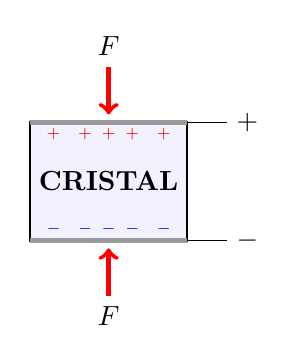
\begin{tikzpicture}[scale=1]
        % Material piezo (bloque)
        \draw[thick, fill=blue!5] (0,0) rectangle (2,1.5);
        \node at (1,0.75) {\textbf{CRISTAL}};
        
        % Electrodos
        \draw[ultra thick, gray!80] (0,1.5) -- (2,1.5) coordinate (top);
        \draw[ultra thick, gray!80] (0,0) -- (2,0) coordinate (bot);
        
        % Flechas de fuerza
        \draw[ultra thick, red, ->] (1,2.2) -- (1,1.6) node[above, pos=0, black] {$F$};
        \draw[ultra thick, red, <-] (1,-0.1) -- (1,-0.7) node[below, pos=1, black] {$F$};
        
        % Cargas generadas
        \foreach \x in {0.3, 0.7, 1, 1.3, 1.7} {
            \node[red] at (\x, 1.35) {\tiny $+$};
            \node[blue] at (\x, 0.15) {\tiny $-$};
        }
        
        % Terminales
        \draw (top) -- (2.5,1.5) node[right] {$+$};
        \draw (bot) -- (2.5,0) node[right] {$-$};
    \end{tikzpicture}
    \caption[Principio de transducción piezoeléctrica.]{Principio de transducción piezoeléctrica. La fuerza $F$ desequilibra los dipolos internos, induciendo cargas superficiales que son captadas por los electrodos metálicos.}\label{fig:celda_piezo}
\end{marginfigure}

\marginnote{\textbf{Materiales Comunes Piezoeléctricos:} \\
    \textbf{Cuarzo:} Excelente linealidad y estabilidad, pero baja sensibilidad. \\
    \textbf{PZT (Cerámica):} Alta sensibilidad (\qty{300}{\pico C/\newton}), muy usado en ultrasonidos. \\
    \textbf{PVDF:} Polímero flexible, ideal para medir impactos en superficies curvas.
}

\subsection{Modelo Eléctrico Equivalente}
Para un ingeniero electrónico, el sensor se modela como una fuente de corriente proporcional a la derivada de la fuerza (ya que $i = dq/dt$) en paralelo con la capacidad propia del cristal $C_s$ y su resistencia de aislamiento $R_s$, como se presenta en la Figura~\ref{fig:modelo_equivalente_piezo}.

\begin{marginfigure}
    \centering
    \shorthandoff{>}
    \begin{tikzpicture}[american, scale=1]
        \ctikzset{resistors/scale=0.7, capacitors/scale=0.7}
        % Fuente de carga/corriente
        \draw (0,0) to[isource, l={$i = d\frac{dq}{dt}$}] (0,2) -- (1,2);
        \draw (1,2) to[C, l=$C_s$, *-*] (1,0);
        \draw (1,2) -- (2,2) to[R, l=$R_s$, *-*] (2,0);
        \draw (0,0) -- (3,0);
        \draw (2,2) -- (3,2) to[short, -o] (3.5,2) node[right] {$V_{out}$};
        \draw (3,0) to[short, -o] (3.5,0);
    \end{tikzpicture}
    \caption[Circuito equivalente del sensor piezoeléctrico.]{Circuito equivalente de un sensor piezoeléctrico. $C_s$ es la capacidad interna (\qtyrange{10}{1000}{\pico F}) y $R_s$ es la resistencia de fugas, que debe ser muy elevada ($>\qty{10}{\giga\Omega}$).}\label{fig:modelo_equivalente_piezo}
\end{marginfigure}

Puesto que $R_s$ es finita, cualquier carga generada terminará por drenarse a través de ella. Esto implica que los sensores piezoeléctricos \emph{no pueden medir fuerzas estáticas}: la señal decae hacia cero aunque la fuerza permanezca constante.

\subsection{Respuesta en Frecuencia y Error Dinámico}
% Conectar con el amplificador de carga visto en el Cap 5.
Físicamente, el sensor se comporta como un \emph{filtro paso alto}. La frecuencia de corte inferior $f_c$ depende de la constante de tiempo $\tau = R_{eq}C_{eq}$ del sistema. Como se muestra en la Figura~\ref{fig:bode_piezo}, el sensor solo es útil en el rango de frecuencias donde la sensibilidad es plana.

\begin{marginfigure}[3em]
    \centering
    \shorthandoff{>}
    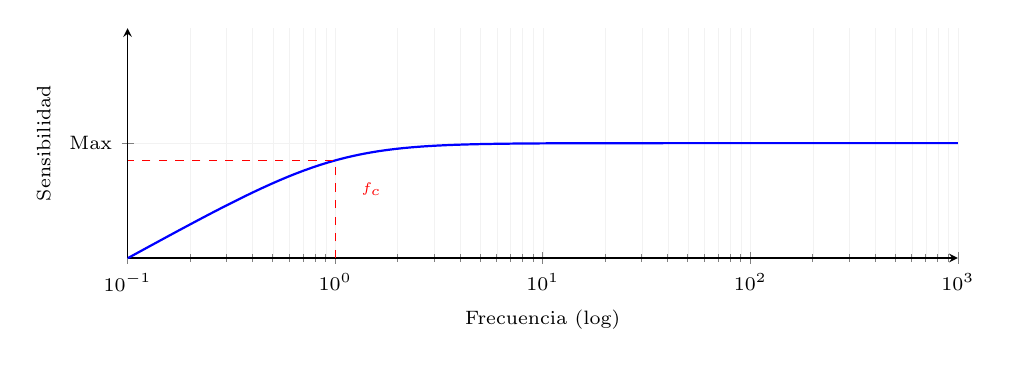
\begin{tikzpicture}
        \begin{axis}[
            width=\linewidth, height=4.5cm,
            xlabel={Frecuencia (log)}, ylabel={Sensibilidad},
            xmode=log, ymode=log,
            xmin=0.1, xmax=1000, ymin=0.1, ymax=10,
            axis lines=left, grid=both,
            grid style={line width=.1pt, draw=gray!10},
            font=\scriptsize,
            xtick={0.1, 1, 10, 100, 1000},
            ytick={1}, yticklabels={Max},
            scaled ticks=false
        ]
            % Curva característica pasa-alto
            \addplot[thick, blue, domain=0.1:1000, samples=100] {1/sqrt(1 + (1/x)^2)};
            \draw[dashed, red] (axis cs:1, 0.1) -- (axis cs:1, 0.707) -- (axis cs:0.1, 0.707);
            \node[red, font=\tiny, anchor=west] at (axis cs:1.2, 0.4) {$f_c$};
        \end{axis}
    \end{tikzpicture}
    \caption[Respuesta en frecuencia cualitativa.]{Respuesta en frecuencia cualitativa. El sensor es insensible a la componente continua. La medida estática es imposible debido a la descarga a través de $R_s$.}\label{fig:bode_piezo}
\end{marginfigure}

\marginnote[2em]{\textbf{Temperatura de Curie:} La temperatura de curie de un material piezoeléctrico es la temperatura a la que el material pierde sus propiedades dipolares permanentemente. En el cuarzo es de \qty{573}{\degree C}, mientras que en cerámicas PZT ronda los \qty{300}{\degree C}.
}

\paragraph{Acondicionamiento: El Amplificador de Carga}
Si conectamos el sensor a un amplificador de tensión convencional, la capacidad del cable ($C_c$) atenuará la señal y hará que la calibración dependa de la longitud del cable ($V = q / (C_s + C_c)$).

Para solucionar esto, se emplea el \emph{Amplificador de Carga} analizado en el Capítulo~\ref{cap:opamps}. Gracias a la tierra virtual, el potencial del cable se mantiene en cero, anulando la carga en $C_c$ y haciendo que la tensión de salida dependa exclusivamente del condensador de realimentación $C_f$:
\begin{equation}
    V_{out} = -\frac{q}{C_f} = -\frac{d \cdot F}{C_f}
\end{equation}

\marginnote{\textbf{Aplicación: Acelerómetros:} 
    Son el uso más común de estos sensores. Una masa sísmica presiona el cristal ante una aceleración $a$, generando una fuerza $F=m \cdot a$. Permiten medir vibraciones de hasta \qty{50}{\kilo\hertz} en motores y estructuras.
}


\section{Otros Sensores Generadores}\label{sec:otros_generadores}
Para completar el estudio de los sensores generadores, se analizan aquellos dispositivos que transforman la energía radiante y la energía cinética directamente en señales eléctricas utilizables por un sistema de instrumentación.

\subsection{Sensores Fotovoltaicos (Células solares)}
Se basan en el efecto fotovoltaico, el cual ocurre en una unión PN de material semiconductor (típicamente silicio) cuando es impactada por fotones con energía superior al \textit{bandgap} del material. A diferencia de las fotorresistencias (LDR) analizadas en capítulos previos, estos sensores no modulan una resistencia, sino que actúan como una fuente real de corriente.

Como se ilustra en la Figura~\ref{fig:celda_fotovoltaica}, la incidencia de luz genera pares electrón-hueco en la zona de deplexión de la unión. En aplicaciones de instrumentación de precisión (como fotómetros), el sensor debe operar en \emph{modo de cortocircuito}. En esta configuración, la corriente generada $I_{ph}$ presenta una relación lineal con la iluminancia $E$ recibida:

\begin{equation}\label{eq:corriente_luz}
    I_{ph} \approx k \cdot E
\end{equation}

\begin{marginfigure}[0em]
    \centering
    \shorthandoff{>}
    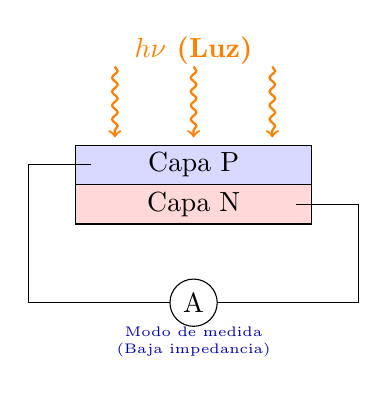
\begin{tikzpicture}[scale=1]
        % Unión PN
        \draw[fill=blue!15] (0,0.5) rectangle (3,1); \node at (1.5,0.75) {Capa P};
        \draw[fill=red!15] (0,0) rectangle (3,0.5); \node at (1.5,0.25) {Capa N};
        
        % Fotones (h*nu)
        \foreach \x in {0.5, 1.5, 2.5} {
            \draw[orange, ->, thick, decoration={snake, amplitude=1pt, segment length=5pt}, decorate] (\x, 2) -- (\x, 1.1);
        }
        \node[orange, font=\bfseries] at (1.5, 2.2) {$h\nu$ (Luz)};
        
        % Circuito
        \draw (0.2,0.75) -- (-0.6,0.75) -- (-0.6,-1) coordinate (bot_left);
        \draw (2.8,0.25) -- (3.6,0.25) -- (3.6,-1) coordinate (bot_right);
        
        % Amperímetro
        \draw (1.5, -1) circle (0.3) node {A};
        \draw (bot_left) -- (1.2, -1);
        \draw (bot_right) -- (1.8, -1);
        
        \node[blue!70!black, font=\tiny, align=center] at (1.5, -1.5) {Modo de medida\\(Baja impedancia)};
    \end{tikzpicture}
    \caption[Principio del sensor fotovoltaico.]{Operación de un sensor fotovoltaico. La energía de los fotones genera portadores de carga que dan lugar a la corriente de fotodiodo $I_{ph}$.}\label{fig:celda_fotovoltaica}
\end{marginfigure}

\marginnote[0em]{
    \textbf{Respuesta Espectral:} La sensibilidad no es uniforme para todos los colores. Los sensores de silicio tienen su pico de respuesta en el infrarrojo cercano (aprox. \qty{900}{nm}). Para medir iluminancia visible, se requieren filtros ópticos que ajusten la respuesta a la curva fotópica del ojo humano.
}

\subsection{Sensores Electrodinámicos (Velocímetros)}

Estos sensores aprovechan la \emph{Ley de Inducción de Faraday} para medir la velocidad mecánica sin necesidad de alimentación. Constan de un imán permanente y un bobinado móvil. Cuando la bobina se desplaza a una velocidad $v$ dentro del campo magnético uniforme $B$, se induce una tensión proporcional a dicha velocidad:

\begin{equation}\label{eq:fem_velocidad}
    e = B \cdot l \cdot v
\end{equation}
donde $l$ es la longitud total del conductor del bobinado expuesto al flujo. Como se observa en la Figura~\ref{fig:velocimetro}, el sensor genera una tensión alterna si el movimiento es vibratorio.

\begin{marginfigure}
    \centering
    \shorthandoff{>}
    \begin{tikzpicture}[american, scale=0.9, font=\scriptsize]
        % Imán fijo
        \draw[thick, fill=gray!10] (0,0) rectangle (0.8,2);
        \node[red] at (0.4, 1.5) {\textbf{N}};
        \node[blue] at (0.4, 0.5) {\textbf{S}};
        
        % Líneas de campo B
        \foreach \y in {0.6, 1, 1.4} {
            \draw[green!60!black, ->, dashed] (0.9, \y) -- (2.3, \y);
        }
        \node[green!60!black, font=\tiny] at (1.6, 1.7) {$\vec{B}$};

        % Bobina móvil (Vibrante)
        \draw[ultra thick, orange!80!black] (2, 0.3) rectangle (2.4, 1.7);
        \foreach \y in {0.5, 0.8, 1.1, 1.4} {
            \draw[orange] (2, \y) -- (2.4, \y);
        }
        
        % Flecha de velocidad
        \draw[ultra thick, blue, <->, >=stealth] (2.2, 2) -- (2.2, 2.6) node[above] {$\vec{v}(t)$};
        
        % Salida
        \draw (2.2, 0.3) -- (2.2, -0.4) to[short, -o] (3, -0.4) node[right] {$V_{out} \propto v$};
    \end{tikzpicture}
    \caption[Esquema de un sensor electrodinámico.]{Transductor electrodinámico. La tensión de salida es una réplica exacta de la velocidad instantánea del objeto, muy común en sismometría y monitorización de turbinas.}\label{fig:velocimetro}
\end{marginfigure}

\marginnote{\textbf{Limitación en DC:} Al igual que los piezoeléctricos, los sensores electrodinámicos son incapaces de realizar medidas estáticas. Si la velocidad es nula, el flujo magnético no cambia y la tensión de salida cae a cero, independientemente de la posición del sensor.
}


\section{Resumen y Comparativa}\label{sec:resumen_generadores}

Para finalizar el capítulo, la Tabla~\ref{tab:resumen_generadores} presenta una comparativa técnica de las tecnologías generadoras analizadas. La principal ventaja competitiva de estos sensores es su \emph{autonomía energética}, extrayendo la energía necesaria para la señal directamente de la magnitud física medida.

\begin{table}[ht]
    \centering
    \small
    \caption{Comparativa de sensores generadores. Nótese la diversidad de señales de salida (tensión, carga o corriente), lo que exige etapas de acondicionamiento específicas para cada tecnología.}\label{tab:resumen_generadores}
    \setlength{\tabcolsep}{1pt}
    \begin{tabularx}{\linewidth}{l X X X}
        \toprule
        \textbf{Tipo} & \textbf{Efecto Físico} & \textbf{Salida Típica} & \textbf{Aplicación Principal} \\
        \midrule
        \emph{Termopar} & Seebeck & Tensión (mV) & Criogenia y fundiciones. \\
        \emph{Piezoeléctrico} & Polarización & Carga (pC) & Aceleración y ultrasonidos. \\
        \emph{Fotovoltaico} & Fotogeneración & Corriente ($\mu$A) & Medida de iluminancia (lux). \\
        \emph{Electrodinámico} & Inducción & Tensión (V) & Velocidad de vibración. \\
        \bottomrule
    \end{tabularx}
    
\end{table}

\marginnote{\textbf{Conclusión de Diseño:} Mientras que los sensores pasivos (Capítulos 3 y 4) suelen requerir puentes de medida para detectar variaciones pequeñas, los generadores exigen amplificadores con \textbf{impedancia de entrada extremadamente alta} o sistemas de \textbf{compensación de referencia} para no degradar la señal original.
}

\cleardoublepage